\documentclass{article}
\usepackage{booktabs}
\usepackage{multirow}
\usepackage{graphicx}

\title{Lab09 Report}
\author{ Group-33 }
\date{}

\begin{document}
\maketitle
\pagenumbering{gobble}

\begin{table}[h!]
\begin{center}

 \begin{tabular}{*{3}{c}}
\toprule
Group Name & Name & Roll No.\\
\midrule
\multirow{3}{*}{Anonymous} & Deep & 140050002 \\
  & Kapil & 140050006 \\
  & Mohit & 140050015 \\
\bottomrule
\end{tabular} 
 
\end{center}
\end{table}

\newpage

\section{Observations}
\subsection{debugVersion}
originally in program running in part,a-debug was running slow. call graph using gprof showed that debug\_draw\_t::DrawSolidCircle function was consuming sufficiently large portion of time. So to make code run fast we checked that function and line 102 of render.cpp in src folder contained for loop running 3000000 times. Code was optimised by commenting this line.
\newline
\newline
\newline
Top 5 functions are :
\begin{enumerate}
	\item operator*(float, b2Vec2 const\&)
	\item operator-(b2Vec2 const\&, b2Vec2 const\&)
	\item b2ContactSolver::SolveVelocityConstraints()
	\item b2Vec2::b2Vec2(float, float)
	\item b2Cross(float, b2Vec2 const\&)
\end{enumerate}

\subsection{releaseVersion}
flag -O3 was added in CPPFLAGS to optimise program.
\newline
Top 5 functions are :
\begin{enumerate}
	\item debug\_draw\_t::DrawSolidCircle(b2Vec2 const\&, float, b2Vec2 const\&, b2Color const\&)
	\item b2CollideEdgeAndPolygon(b2Manifold*, b2EdgeShape const*, b2Transform const\&, b2PolygonShape const*, b2Transform const\&)
	\item b2ContactManager::Collide()
	\item b2StackAllocator::Free(void*)
	\item b2World::Solve(b2TimeStep const\&)
\end{enumerate}

\newpage
\section{Images}
\subsection{debugVersion.png}
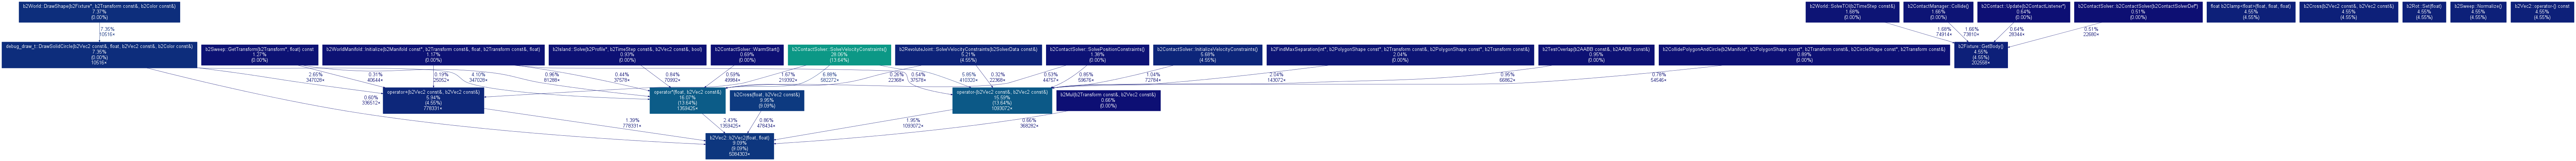
\includegraphics[width=\linewidth]{debugVersion.png}
Note that image is also exists in basecode's doc folder


\subsection{releaseVersion.png}
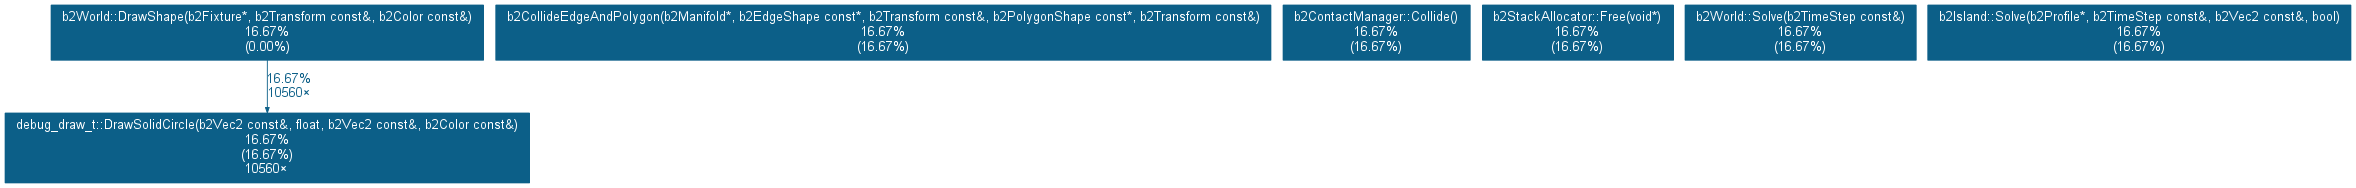
\includegraphics[width=\linewidth]{releaseVersion.png}
Note that image is also exists in basecode's doc folder


\end{document}